\documentclass[10pt]{article}
\usepackage[utf8]{inputenc}
\usepackage[brazil]{babel}
\usepackage{ae}
\usepackage{amssymb,amsmath,amssymb,graphicx,fancyhdr,epsfig,psfrag,tabularx,float,caption}
\usepackage[paperwidth=210mm,paperheight=297mm]{geometry}
\usepackage{times}
\usepackage{textcomp}
\usepackage[table]{xcolor}
\usepackage{colortbl}
\usepackage{url}
\usepackage{listings} % inclusion of source code
\usepackage{hyperref} % clean URLs

% the following is needed for syntax highlighting
\usepackage{color}

\definecolor{dkgreen}{rgb}{0,0.6,0}
\definecolor{gray}{rgb}{0.5,0.5,0.5}
\definecolor{mauve}{rgb}{0.58,0,0.82}

\lstset{ %
  language=Java,                  % the language of the code
  basicstyle=\footnotesize,       % the size of the fonts that are used for the code
  numbers=left,                   % where to put the line-numbers
  numberstyle=\tiny\color{gray},  % the style that is used for the line-numbers
  stepnumber=1,                   % the step between two line-numbers. If it's 1, each line 
                                  % will be numbered
  numbersep=5pt,                  % how far the line-numbers are from the code
  backgroundcolor=\color{white},  % choose the background color. You must add \usepackage{color}
  showspaces=false,               % show spaces adding particular underscores
  showstringspaces=false,         % underline spaces within strings
  showtabs=false,                 % show tabs within strings adding particular underscores
  frame=single,                   % adds a frame around the code
  rulecolor=\color{black},        % if not set, the frame-color may be changed on line-breaks within not-black text (e.g. commens (green here))
  tabsize=4,                      % sets default tabsize to 2 spaces
  captionpos=b,                   % sets the caption-position to bottom
  breaklines=true,                % sets automatic line breaking
  breakatwhitespace=false,        % sets if automatic breaks should only happen at whitespace
  title=\lstname,                 % show the filename of files included with \lstinputlisting;
                                  % also try caption instead of title
  keywordstyle=\color{blue},          % keyword style
  commentstyle=\color{dkgreen},       % comment style
  stringstyle=\color{mauve},         % string literal style
  escapeinside={\%*}{*)},            % if you want to add a comment within your code
  morekeywords={*,...}               % if you want to add more keywords to the set
}

% \newcommand{\blue}{\textcolor{blue}}
% \newcommand{\blue}{}
\hyphenation{pro-ble-mas}

\begin{document}

\selectlanguage{brazil}

\begin{large}
	\begin{center}
		\textbf{MC302} \\
		Primeiro semestre de 2017 \\ \vspace{0.5cm}
		\textbf{Laboratório 1}
	\end{center}
\end{large}
\vspace{0.25cm}
\noindent \textbf{Professor(a):} Esther Colombini (esther@ic.unicamp.br) \\
\textbf{PEDs:} Elisangela Santos (ra149781@students.ic.unicamp.br), Lucas Faloni (lucasfaloni@gmail.com), Lucas David (lucasolivdavid@gmail.com), Wellington Moura (wellington.tylon@hotmail.com) \\
\textbf{PAD:} Igor Torrente (igortorrente@hotmail.com) \\
\noindent \textbf{Professor(a):} Fábio Luiz Usberti (fusberti@ic.unicamp.br) \\
\textbf{PEDs:} Natanael Ramos (naelr8@gmail.com), Rafael Arakaki (rafaelkendyarakaki@gmail.com) \\
\textbf{PAD:} Bleno Claus (blenoclaus@gmail.com) \\

\hrule \hrule

\section{Objetivo}

O objetivo desta atividade consiste na prática de Hierarquias de generalização/especialização e Herança Simples e Múltipla.
Por meio de encapsulamento e herança novas técnicas podem ser adicionadas as classes. Enquanto a herança é um poderoso mecanismo de especialização, o polimorfismo oferece um mecanismo para a generalização. No Java uma subclasse somente pode exttender diretamente uma outra subclasse, não sendo permitido a herança múltipla, como ocorre em C++. Ou seja, uma determinada classe em Java pode implementar múltiplas interfaces e fazer uso de agregação para responder por chamadas a métodos que tecnicamente só poderiam acontecer se existisse a "herança múltipla".
Nesta aula treinaremos especialização e heranças. Interfaces e generalização serão assuntos futuros.

\section{Atividade}
Continuaremos trabalhando com classes baseadas no jogo chamado Hearthstone\footnote{http://us.battle.net/hearthstone/pt} \textcopyright.Nesta atividade o principal foco será a familiarização com generalização e herança em java e a programação da classe chamada \textbf{Carta} . Crie um projeto chamado Lab4. No projeto crie os mesmos pacotes da aula passada com.seuPrimeiroNome.Util e com.seuPrimeiroNome.base. Cole a classe CartaLacaio (utilizada no Lab3), a classe CartaMagia (utilizada no Lab2), a classe Baralho (utilizada no Lab3) e a classe BaralhoArrayList dentro do projeto no pacote base.
No pacote Util cole a classe Util.java.


\section{Classe Carta}
Crie a classe Carta no pacote base com os seguintes atributos:
A classe Carta deve ter os seguintes atributos:
\begin{itemize}
    \item ID (número inteiro)
    \item nome (cadeia de caracteres - \emph{String})
    \item tipo (TipoCarta) - Enum\footnote{Enumeração será assunto dos próximos capitulos, portanto não usaremos este atributo agora} \textcopyright: TipoCarta.LACAIO, TipoCarta.MAGIA
    \item ataque (número inteiro)
    \item vida (número inteiro)
    \item vidaMesa (número inteiro)
    \item mana (número inteiro)
    \item magiaTipo (TipoMagia) - Enum\footnote{Enumeração será assunto dos próximos capitulos, portanto não usaremos este atributo agora} \textcopyright: TipoMagia.ALVO, TipoMagia.AREA
     \item magiaDano (número inteiro)
    \item turno (número inteiro)
\end{itemize}

O exemplo abaixo apresenta a declaração da classe Carta e seus atributos. Note que todas as variáveis são declaradas como privadas (\textbf{private}). Note também a implementação dos métodos de acesso get() e set(), esses métodos são comumente utilizados na linguagem Java para acessar os atributos dos objetos.

\lstinputlisting[language=Java]{Carta.java}

Além disso a classe Carta deve conter um método construtor, o método construtor deve receber como argumentos os atributos para inicializar o objeto. Para ilustrar esse conceito melhor, veja o exemplo abaixo.

\lstinputlisting[language=Java]{MetodoConstrutor.java}

Também é necessário que a classe Carta possua uma função \textbf{toString()} que devolve uma String contendo uma descrição geral dos atributos da carta. Veja o exemplo abaixo:

\lstinputlisting[language=Java]{toString.java}

Como já aprendemos são utilizados os métodos de get e set. Precisamos programar estes métodos antes de utilizá-los,  para cada atributo da classe Carta deve existir um método get e set correspondente. O formato do método toString() a ser implementado é aquele que ja aprendemos.

Faça a implementação do método \textbf{construtor}, métodos \textbf{get()} e \textbf{set()} de todos os atributos e do método \textbf{toString()} para a classe \textbf{Carta}.

\section{Herança}
\begin{figure}[ht]
	\centering
	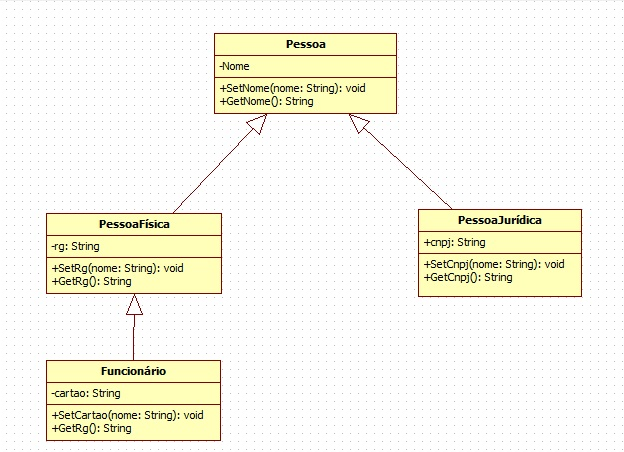
\includegraphics[width=0.95\textwidth]{Exemplo_HierarquiaClasses.jpg}
	\caption{Exemplo de Hierarquia de Classes - Especialização}
	\label{fig:hieraqcollection}
\end{figure}

Diferentes tipos de classes podem ter algo em comum entre elas. Por exemplo diferentes tipos de pessoas podem ter as mesmas característica (nome, sobrenome), a esta classe podemos chamar classe Pessoa. Classes mais especializadas podem herdam os mesmos atributos da classe Pessoa e podem ter atributos não comtemplados na classe principal (denominada superclasse).Por exemplo: A classe PessoaJuridica pode terá o atributo nome e cnpj, nome foi herdado mais cnpj pertence somente a esta classe. Observe na figura 1, o diagrama de hierarquia de classes especializadas. Veja a seguir o código do diagrama de hierarquia de classes, demonstrado na figura 1.

\lstinputlisting[language=Java]{Pessoa.java}

\lstinputlisting[language=Java]{PessoaJuridica.java}

\lstinputlisting[language=Java]{PessoaFisica.java}

\lstinputlisting[language=Java]{Funcionario.java}


\subsection{Adicionando Herança}
Para que a classe especializada (denominada subclasse) consiga herdar todas as características da classe original (denominada superclasse), é necessário que a subclasse seja acrescida da palavra {\itshape Extends}. Veja o exemplo a seguir:

\lstinputlisting[language=Java]{Extends.java}

\subsection{Construtores das classes especializada (denominada subclasse)}
As subclasses (classes especializadas) não herdam os construtores da superclasse (classe original), então é necessário chamar explicitamente o construtor da superclasse. Isso acontece através do comando {\itshape super}. Os parâmetros necessários são passados dentro dos parênteses que seguem essa palavra-chave ({\itshape super}). Veja o exemplo a seguir:

\lstinputlisting[language=Java]{construtor.java}

\section{Tarefas}

\begin{itemize}
	\item Modifique a classse CartaLacaio e CartaMagia para que elas tenham todos os atributos e características da classe Carta (denominada superclasse).
	\item Refaça a programação dos métodos construtores das classes CartaLacaio e CartaMagia, de acordo com o conceito de herança.
	\item Refaça a programação dos métodos get e set das classes CartaLacaio e CartaMagia.
\end{itemize}

\section{Submissão}

Para submeter a atividade utilize o Moodle (\url{https://www.ggte.unicamp.br/ea}). Salve os arquivos dessa atividade em um arquivo comprimido no formato .tar.gz e nomeie-o \textbf{Lab1-000000.tar.gz} trocando '000000' pelo seu número de RA. Submeta o arquivo na seção correspondente para esse laboratório no moodle da disciplina MC302.

\end{document}
% end of file template.tex